\section{Analisi dei risultati}
\label{cap:performance-analysis}

\subsection{Domanda \#1}
\label{sec:question-1}

\begin{displayquote}
Eseguite i tre algoritmi che avete implementato (Held-Karp,
euristica costruttiva e 2-approssimato) sui 13 grafi del dataset.
Mostrate i risultati che avete ottenuto in una tabella come quella
sottostante. Le righe della tabella corrispondono alle istanze del
problema. Le colonne mostrano, per ogni algoritmo, il peso della
soluzione trovata, il tempo di esecuzione e l'errore relativo
calcolato come $(SoluzioneTrovata-SoluzioneOttima)/SoluzioneOttima$.
Potete aggiungere altra informazione alla tabella che ritenete
interessanti.
\end{displayquote}

Per leggibilità la tabella richiesta è stata suddivisa nelle tabelle
\ref{table:held-karp-runtime-accuracy},
\ref{table:mst2approx-runtime-accuracy},
\ref{table:closest-insertion-runtime-accuracy},
una per algoritmo.

\begin{table}[h]
    \centering

    \begin{tabular}{lrrrr}
    \toprule
    \multicolumn{2}{c}{ } & \multicolumn{3}{c}{Held Karp} \\
    \hline
    Instance & Exact & Solution &   Time (ms) &   Error (\%) \\
    \hline
    burma14.tsp   &     3323 &   3323           &          94 &        0    \\
    ulysses16.tsp &     6859 &   6859           &         393 &        0    \\
    ulysses22.tsp &     7013 &   7013           &       75295 &        0    \\
    eil51.tsp     &      426 &    986           &      126289 &      131.46 \\
    berlin52.tsp  &     7542 &  17441           &      126570 &      131.25 \\
    kroA100.tsp   &    21282 & 167464           &      128452 &      686.88 \\
    kroD100.tsp   &    21294 & 149007           &      128377 &      599.76 \\
    ch150.tsp     &     6528 &  48362           &      128392 &      640.84 \\
    gr202.tsp     &    40160 &  55127           &      128389 &       37.27 \\
    gr229.tsp     &   134602 & 176922           &      128344 &       31.44 \\
    pcb442.tsp    &    50778 & 512263           &      128303 &      908.83 \\
    d493.tsp      &    35002 & 321918           &      128277 &      819.71 \\
    dsj1000.tsp   & 18659688 &      5.46817e+08 &      128450 &     2830.47 \\
    \bottomrule
    \end{tabular}

    \caption{Tempo di esecuzione e errore introdotto da Held \& Karp rispetto alle istanze.}
    \label{table:held-karp-runtime-accuracy}
\end{table}

\begin{table}[h]
    \centering

    \begin{tabular}{lrrrr}
    \toprule
    \multicolumn{2}{c}{ } & \multicolumn{3}{c}{MST 2 Approximation} \\
    \hline
    Instance & Exact & Solution &   Time (ms) &   Error (\%) \\
    \hline
    burma14.tsp   &     3323 &   4258           &          33 &       28.14 \\
    ulysses16.tsp &     6859 &   7857           &          35 &       14.55 \\
    ulysses22.tsp &     7013 &   8377           &          36 &       19.45 \\
    eil51.tsp     &      426 &    563           &          36 &       32.16 \\
    berlin52.tsp  &     7542 &  10402           &          36 &       37.92 \\
    kroA100.tsp   &    21282 &  30032           &          36 &       41.11 \\
    kroD100.tsp   &    21294 &  28467           &          36 &       33.69 \\
    ch150.tsp     &     6528 &   9116           &          34 &       39.64 \\
    gr202.tsp     &    40160 &  52967           &          38 &       31.89 \\
    gr229.tsp     &   134602 & 178434           &          37 &       32.56 \\
    pcb442.tsp    &    50778 &  74254           &          42 &       46.23 \\
    d493.tsp      &    35002 &  45669           &          44 &       30.48 \\
    dsj1000.tsp   & 18659688 &      2.57036e+07 &          69 &       37.75 \\
    \bottomrule
    \end{tabular}

    \caption{Tempo di esecuzione e errore introdotto da MST 2 Approximation rispetto alle istanze}
    \label{table:mst2approx-runtime-accuracy}
\end{table}

\begin{table}[h]
    \centering

    \begin{tabular}{lrrrr}
    \toprule
    \multicolumn{2}{c}{ } & \multicolumn{3}{c}{Farthest Insertion} \\
    \hline
    Instance & Exact & Solution &   Time (ms) &   Error (\%) \\
    \hline
    burma14.tsp   &     3323 &   3511.5         &          35 &        5.67 \\
    ulysses16.tsp &     6859 &   7377           &          37 &        7.55 \\
    ulysses22.tsp &     7013 &   7703.5         &          36 &        9.85 \\
    eil51.tsp     &      426 &    487           &          36 &       14.32 \\
    berlin52.tsp  &     7542 &   9047           &          37 &       19.95 \\
    kroA100.tsp   &    21282 &  25842           &          37 &       21.43 \\
    kroD100.tsp   &    21294 &  25230           &          36 &       18.48 \\
    ch150.tsp     &     6528 &   8072           &          40 &       23.65 \\
    gr202.tsp     &    40160 &  48011           &          46 &       19.55 \\
    gr229.tsp     &   134602 & 158933           &          68 &       18.08 \\
    pcb442.tsp    &    50778 &  60235.5         &         141 &       18.63 \\
    d493.tsp      &    35002 &  41870.5         &         175 &       19.62 \\
    dsj1000.tsp   & 18659688 &      2.27984e+07 &        1110 &       22.18 \\
    \bottomrule
    \end{tabular}

    \caption{Tempo di esecuzione e errore introdotto da Closest Insertion rispetto alle istanze}
    \label{table:closest-insertion-runtime-accuracy}
\end{table}

Una lettura più chiara dell'errore di approssimazione è invece
fornita dai grafici
\ref{fig:heldkarp-mst2approx-closestinsertion-accuracy-error-52-nodes}
 e \ref{fig:heldkarp-mst2approx-closestinsertion-accuracy-error}.
\'E possibile notare come nel
secondo grafico l'errore di approssimazione di HeldKarp diventi
praticamente impredicibile, tendendo comunque a crescere con la
dimensione del grafo. Nel primo grafico invece è facile vedere
come l'algoritmo MST2Approximation sia l'unico ad avere errore
di approssimazione anche su taglie dell'input piccole,
come ci si aspettava.

\begin{figure}[H]
    \centering

    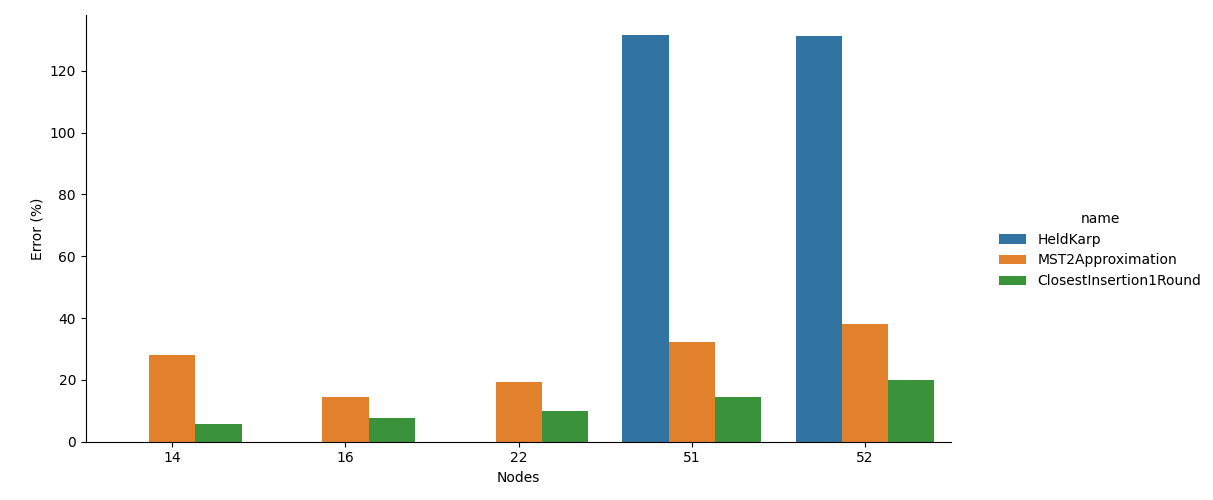
\includegraphics[width=0.9\textwidth]{./images/HeldKarp_vs_MST2Approximation_vs_ClosestInsertion1Round__approximation_error__limited_to_52_nodes_.png}

    \caption{Confronto dell'errore introdotto da HeldKarp, MST2Approximatione e ClosestInsertion rispetto al numero di nodi (da 14 a 52)}
    \label{fig:heldkarp-mst2approx-closestinsertion-accuracy-error-52-nodes}
\end{figure}

\begin{figure}[H]
    \centering

    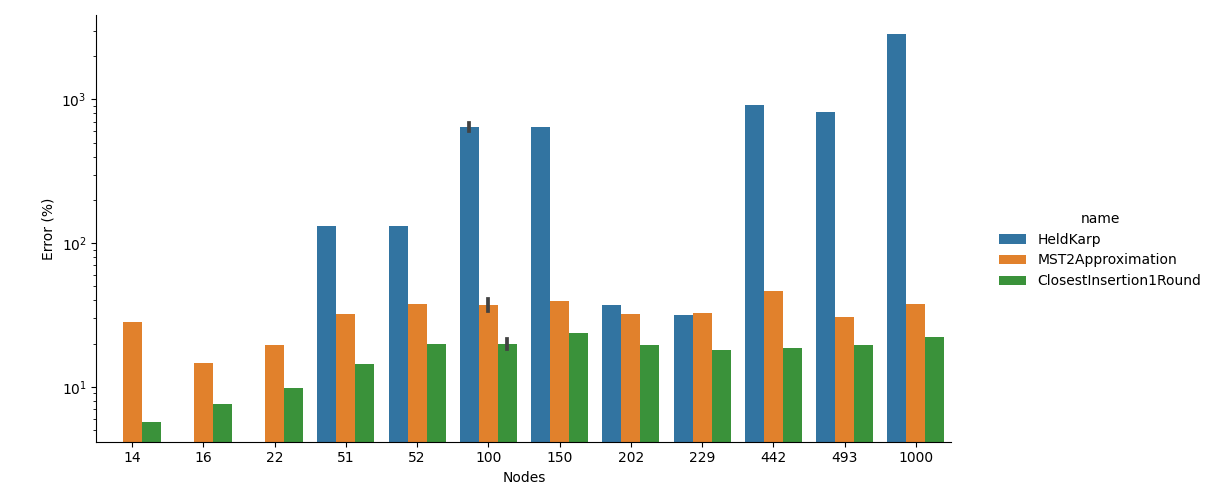
\includegraphics[width=0.9\textwidth]{./images/HeldKarp_vs_MST2Approximation_vs_ClosestInsertion1Round__approximation_error__y_log_scaled_.png}

    \caption{Confronto dell'errore introdotto da HeldKarp, MST2Approximation e ClosestInsertion rispetto al numero di nodi (errore in scala logaritmica)}
    \label{fig:heldkarp-mst2approx-closestinsertion-accuracy-error}
\end{figure}

Il grafico che mostra i tempi di esecuzione non è stato inserito
in quanto ritenuto veramente poco informativo: HeldKarp va in
timeout dopo i ventidue nodi (con il timeout fissato a due minuti),
mentre gli altri due algoritmi terminano in poco più di un secondo
su grafi di mille nodi.

\subsection{Domanda \#2}
\label{sec:question-2}

\begin{displayquote}
Commentate i risultati che avete ottenuto: come si comportano gli
algoritmi rispetti alle varie istanze? C'è un algoritmo che riesce
sempre a fare meglio degli altri rispetto all'errore di
approssimazione? Quale dei tre algoritmi che avete implementato è
più efficiente?
\end{displayquote}


\noindent Gli algoritmi che abbiamo deciso di analizzare, come scritto
nella sezione \ref{sec:question-1}, sono HeldKarp, MST2Approximation e
ClosestInsertion. I dati riportati dalle tabelle e dai grafici sono di
facile lettura. Di seguito sono riportate alcune osservazioni sui
risultati ottenuti.

\begin{itemize}
    \item L'algoritmo di HeldKarp, anche per taglie piccole dell'input
      va in timeout e sopra i 22 nodi inizia a restituire delle
      soluzioni parziali che si discostano molto dalla soluzione
      esatta. Questo fenomeno aumenta di molto soprattutto su taglie
      grosse dell'input, anche se è possibile notare un'inversione di
      tendenza per le istanze \emph{gr202} e \emph{gr229}, dove
      l'errore introdotto da Held \& Karp è simile a quello di
      MST2Approximation. \'E possibile ipotizzare che questo fenomeno
      si verifichi per via della distribuzione dei nodi e quindi del
      valore che gli archi assumono, mi rimane un evento limitato, tra
      l'altro a due istanze la cui sorgente di dati è la stessa. \\

    \item L'algoritmo MST2Approximation introduce un errore di
      approssimazione non trascurabile anche su taglie piccole
      dell'input, ma ciò compensa con il tempo di esecuzione
      dell'algoritmo. Per dare un'idea, il tempo di esecuzione
      migliore di MST2Approximation sul grafo di 1000 nodi è di 69
      millisecondi, il chè rende questo algoritmo il più efficiente
      tra i tre confrontati. L'approssimazione introdotta, a parte
      l'oscillazione iniziale, rimane pressoché costante, intorno al
      30/40\% di errore rispetto alla soluzione ottima. Tutto sommato,
      data la semplicità dell'algoritmo, i risultati sono soddisfacenti. \\

    \item L'algoritmo ClosestInsertion che implementa l'euristica
      costruttiva è il vincitore dei nostri benchmark per quanto
      riguarda l'errore di approssimazione. Dai dati raccolti,
      l'algoritmo è in grado di fare sempre meglio di HeldKarp e di
      MST2Approximation. Inoltre l'errore introdotto è relativamente
      basso, infatti, anche per input piuttosto gradi l'errore rimane
      costante intorno al 20\% circa. L'algoritmo ha anche ottimi
      tempi di runtime, fino a 200 nodi il tempo di esecuzione rimane
      confrontabile con quello di MST2Approx, per input più grossi
      invece il tempo cresce fino ad arrivare a più di 1 secondo per
      il grafo con 1000 nodi. \\

    \item Nella sezione \ref{cap:extensions-and-originalities} abbiamo
      descritto altri algoritmi per la risoluzione di TSP che abbiamo
      deciso di approfondire. In particolare, abbiamo verificato
      empiricamente che l'euristica costruttiva FarthestInsertion
      funziona meglio di ClosestInsertion, e anzi, riesce a fare
      meglio per ogni istanza, con un'errore di approssimazione che
      rimane veramente basso. Per ulteriori dettagli si veda la
      sezione \ref{sec:farthest-insertion}. \\
\end{itemize}
